Design of the VNA takes place in two steps: high level architectural design where the functional blocks of the system are determined, followed by detailed design where specific components are chosen to meet the needs of each functional block. 

\subsection{Architecture}
\label{subsec:architecture}
A VNA has four main functional blocks as shown in Figure \ref{fig:keysight_vna_block_diag}: source for stimulus, signal separation, receiving / detecting, and processing / display. Each of these functional blocks plays a key role in the function of a VNA and will be discussed below.
\begin{figure}[H]
	\centering
	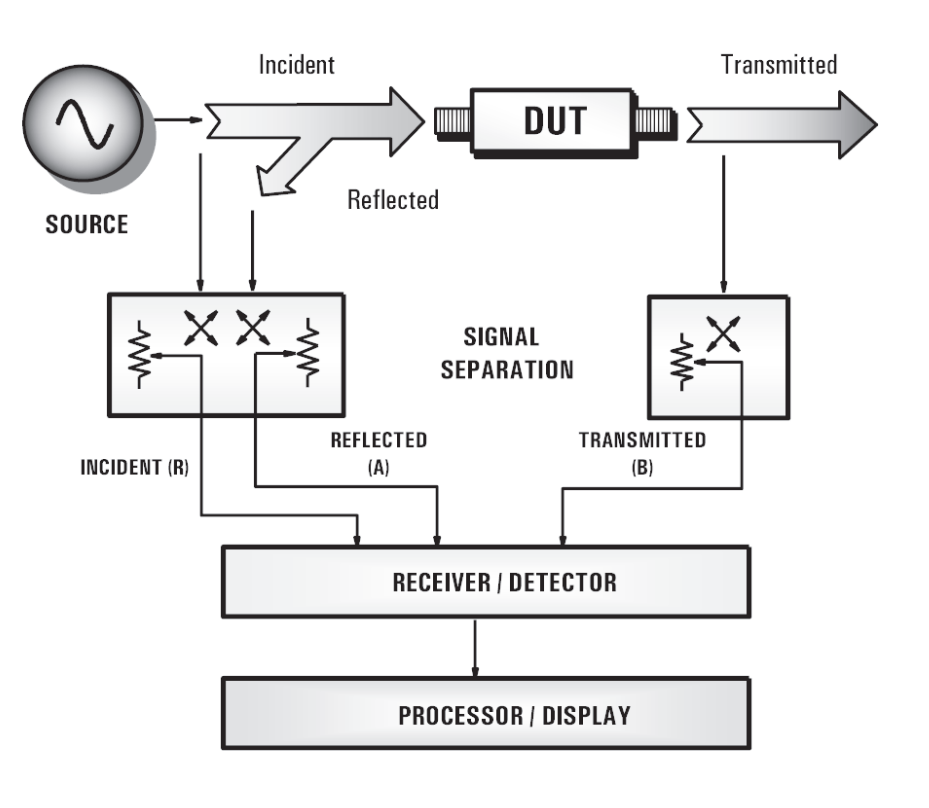
\includegraphics[width=0.6\linewidth]{keysight_vna_block_diag.PNG}
	\caption{Generalised Network Analyser Block Diagram \cite{keysight_vna_basics}}
	\label{fig:keysight_vna_block_diag}
\end{figure}

\subsubsection{Signal Source}
\label{subsec:signal source}
The signal source is the first functional block in the signal path of a VNA, and is responsible for providing the stimulus used for the test system. This source is typically swept over frequency, but can also be swept over power to measure the required parameters. Two primary considerations for the signal source are the phase noise of the signal, which can cause issues with narrow bandwidth measurement if it is too large, and the spectral purity of the signal, which can result in incorrect frequency response measurements if there are spurious tones or harmonics in the output spectrum. 

Typically the signal sources utilise a voltage controller oscillator, which is able to generate continuous wave signals over a wide bandwidth through the use of a PLL to multiply a reference clock to the required frequency. Single chip solutions are available which contain a PLL and multiple VCOs to enable a wide frequency range with only a few external passives, and whilst these PLLs are easy to implement and control, they typically have increased phase noise, harmonics, and spurs compared to a PLL which uses multiple discrete components to close the loop, which is seen on higher end devices where the quality of the output spectrum is key. 

To allow control over the output power level, a power amplifier, programmable attenuator, and power detector can be utilised to provide closed loop control over the output power level. Key features of the source levelling components are that they can provide the required power level over the frequency range being swept, along with not distorting the signal being output by the source. 

\subsubsection{Signal Separation}
\label{subsubsec:signal seperation}
Signal separation is the next functional block in the system, and is utilised to measure a portion of the source for analysis in the receiver / detector subsystem. They are used to measure both the power being output by the source, along with the incident and reflected waves at connections to the DUT. The latter two measurements require directional couplers, as both the incident and reflected waves are on the same PCB trace whilst travelling in opposing directions, and as such high directivity is required to ensure that only the signal travelling in the desired direction is being measured. 

The three most common methods for coupling signals are resistive dividers, which are broadband but lack directivity and have high loss, directional couplers, which have low loss however their coupling and directivity are limited in bandwidth, and directional bridges, which are broadband, can have high directivity, and have lower loss than restive dividers. 

\subsubsection{Receiver / Detector}
\label{subsubsec: receiver detector}
Most vector network analysers utilise a tuned narrowband detector where the RF incident upon the DUT is downconverted to an intermediate frequency, with an ADC sampling the signal and digital signal processing is then preformed to determine the gain and phase of the IF signal. This design results in high sensitivity and dynamic range, along with good harmonic and spurious tone rejection, and a significantly lower noise floor than other methods. However due to the high sample rates of the ADC required to meet the Nyquist sampling frequency of the signal, this method requires a fast sampling ADC, and the corresponding amount of computing power to preform the signal processing to determine the amplitude and phase of the signal, which is comparatively expensive to other methods.  

In scalar network analysers, diode based detectors are often used as they provide a cost effective solution to measuring power. However they are broadband which can result in spurious measurements at unintended frequencies, do not have the sensitivity and dynamic range of a tuned detector, and are only able to measure gain, not phase of a signal. As such they are not suitable for use in a vector network analyser where phase measurements are required.

A third potential receiver utilises the AD8302 from Analog Devices, which is a RF / IF Gain and Phase Detector.\cite{ad8302_datasheet} The AD8302 contains dual demodulating log amplifiers and a phase detector, which generates two analog  voltages which correspond to the gain and phase difference between the input RF signals. This design has the same issues as a diode detector due to utilising diode detectors internally for gain detection, however it resolves the phase measurement issue due to generating phase difference as a second output. There are however some signal processing challenges which need to be overcome with the phase detection, as the output can not differentiate between positive and negative phase, and also has non insignificant log conformance error at small phase differences and higher frequencies. However, given that its cost is between the two other solutions outlined above, it may be a cost effective solution to gain and phase detection if high dynamic range is not required. 

\subsubsection{Processor / Display}
\label{subsubsec:processor display}
The final functional block in a VNA is the processing and display of the received data, where the raw data measured by the receiver is transformed and displayed in various ways which enable the user to make informed decisions about the measurements being taken. 

Depending on the amount of processing required, the compute requirements may vary from multiple custom ASICs for the digital signal processing combined with a Windows install, touch screen, and physical buttons for the application layer, all the way through to a Cortex M0 microcontroller with a small TFT display which handles both the signal processing and display to the user. In recent years, companies such as Tektronix have been rolling out 'headless' devices which utilise the user's computer to handle the application layer, enabling smaller and cheaper test and measurements devices as they no longer require a screen along with the user interface on device. 

\subsubsection{Chosen Architecture} 
\label{subsubsec:chosen architecture}
Taking into account the constraints and specifications in combination with the common architectures outlined above, the desired architecture for the device can be decided so that the scope can be narrowed for detailed design. 
\begin{itemize}
	\item \textbf{Signal Source -} a single chip PLL with integrated VCO would be well suited for the VNA, as the benefits from a single chip solution which is cheaper, takes up less board space, and is easier to configure than a PLL made of discrete components far outweighs the loss of performance which will result the single chip solution. 
	\item \textbf{Signal Separation -} whilst a directional bridge would be ideal as it has high directivity whilst working over a wide frequency range, the desire for all components to be COTS rules this out, as they are typically designed into the PCB and as such would require extensive simulation and testing, even if a reference design such as the work of of N. Drobotun and P. Mikheev in their paper "A 300khz-13.5ghz directional bridge" \cite{resistive_coupler} was to be implemented. As such a directional coupler will be the best option, with the main limitation being the availability of broadband directional couplers in the desired frequency range. 
	\item \textbf{Receiver / Detector -} whilst a tuned narrowband detector would be ideal, the cost of a high sample rate ADC along with a FPGA to do the signal processing would exceed the desired BOM of the VNA. As such, the AD8302 from Analog Devices will form the receiver as it has sufficient performance characteristics whilst being significantly cheaper than a digital front end. 
	\item \textbf{Processor / Display -} given the use of an AD8302 for gain and phase detection, a microcontroller will have sufficient processing power and can be utilised to keep costs low. Furthermore, offloading data processing and visualisation to a host computer will allow for further reduction in cost due to not requiring the extra processing power, display, or user interface controls to be added to the device.
\end{itemize}

\subsection{Detailed Design}
\label{subsec:detailed_design}
With the architecture of the VNA outlined and constraints which influence component selection documented, detailed design of the VNA can begin. The following section outlines key considerations in component choice, low level design details, along with some of the testing and characterisation which was done prior to finalising the first schematic. A block diagram of the system can be found in Figure \ref{fig:vna_block_diag}, with the full schematic for the VNA in Appendix \ref{appen:vna_design_files}.

\subsubsection{LO Generation}
The first part of the RF chain begins with the LO, as it generates the signal used throughout the VNA. As outlined in the architecture section, a single chip solution is desired and resulting from research two primary options were found: ADF4351 from Analog Devices, and the MAX2871 from Maxim. The Table \ref{table:lo_comparison} summaries their specifications. 

\begin{landscape}
	\begin{figure}
		\centering
		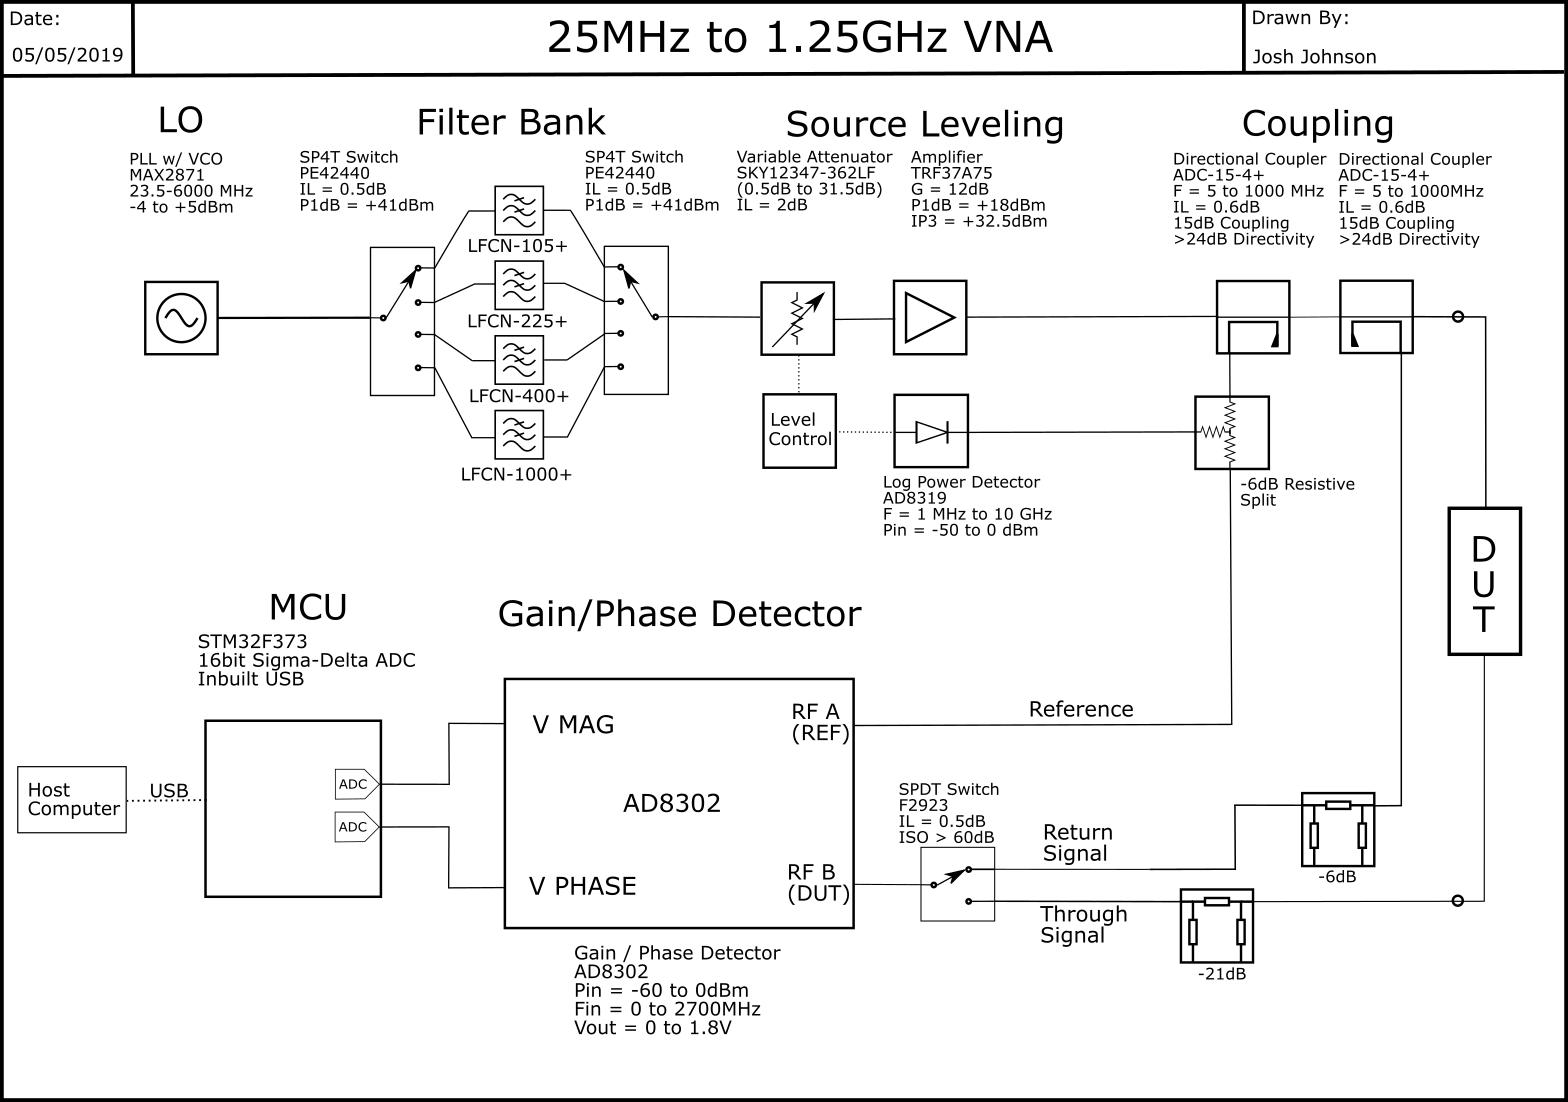
\includegraphics[width=\linewidth]{josh_block_diag.png}
		\caption{Functional Block Diagram of VNA}
		\label{fig:vna_block_diag}
	\end{figure}
\end{landscape}

\begin{table}[H]
	\caption{Comparison of LO generation ICs}
	\label{table:lo_comparison}
	\centering
\begin{tabular}{|c|c|c|}
	\hline
	\multicolumn{1}{|l|}{}          & \textbf{MAX2871} & \textbf{ADF4351} \\ \hline
	\textbf{Frequency Range MHz}    & 23.5 - 6000      & 35 - 4400        \\ \hline
	\textbf{Fractional / Integer N} & Fractional       & Fractional       \\ \hline
	\textbf{Max Output Power (dBm)}   & 5                & 5                \\ \hline
	\textbf{Cost (\$ at Quantity 1)}& 17               & 23             \\ \hline
	\textbf{Example Code}           & No               & Yes              \\ \hline
\end{tabular}
\end{table}
\vspace{-1em}
As can be seen from Table \ref{table:lo_comparison}, the MAX2871 has a wider frequency range, whilst having a lower cost and having the same maximum output power and Fractional-N PLL as the AD4351. The only downside of it for our application is that there is no example code provided by Maxim, and this combined with it's poor data sheet may result in extended firmware development time, whereas Analog Devices provides example code along with an extremely well documented data sheet and application notes. Given there is no cost associated with firmware development and that the goal for the device is to have the widest frequency band at the lowest cost possible, the MAX2871 was chosen due to it's superior specifications. 

\subsubsection{LO Filtering}
\label{subsubsec:lo filtering}
Due to the LO utilising a divided down output for frequencies below 3 GHz, there are significant harmonics in the output signal which need to be filtered out. As will be discussed later, the directional couplers chosen operate up to 1 GHz, and as such filters need to be chosen which operate up to this frequency. Four filters from Mini-Circuits's LFCN series were chosen, with the goal of only frequencies below the second harmonic of a signal being able to pass through, as this would remove most of the unwanted harmonics. In an ideal world this would prevent all harmonics from a fundamental greater than 50 MHz from passing through the RF chain,  however due to the roll off of the filter, along with some poor decisions resulting from not paying enough attention to the data sheets and not fully understanding of the importance of an harmonic free output, the filter selection resulted in issues which will be discussed in \S \ref{sec:implementation}. The chosen filters are tabulated below, along with the frequencies at which 1, 3, and 40 dB of attenuation are measured. 

\begin{table}[H]
	\caption{Selected Filters}
	\label{table:selected_filters}
	\centering
	\begin{tabular}{|c|c|c|c|c|}
		\hline
		\textbf{}               & \textbf{LFCN-105+} & \textbf{LFCN-225+} & \textbf{LFCN-400+} & \textbf{LFCN-1000+} \\ \hline
		\textbf{1 dB IL (MHz)}  & 125                & 250                & 410                & 1100                \\ \hline
		\textbf{3 dB IL (MHz)}  & 180                & 350                & 560                & 1300                \\ \hline
		\textbf{40 dB IL (MHz)} & 265                & 510                & 680                & 1800                \\ \hline
	\end{tabular}
\end{table}
\vspace{-1em}
During the design of the VNA, filters were chosen based off their 1 dB attenuation, as that is the headline figure which Mini-Circuits names their products by. At the time the filter choices were being made, it was unknown that the PLL's output below 3 GHz was divided down, and the significant amount of harmonics this would result from the output waveform being a square wave instead of a sinusoid. In hindsight, now knowing the importance of harmonics being attenuated by more than the $\sim$ 35 dB of dynamic range of the VNA, filters would be chosen based upon their frequency at with 40 dB of insertion loss is measured, as shown by the bottom row of Table \ref{table:selected_filters}. 

For the filters to be switched in and out of the signal path, two SP4T switches capable of functioning down to 25 MHz were required. The PE42440 from pSemi was chosen due to their flat insertion loss across the frequency band of interest, along with low price. 

\subsubsection{LO Levelling}
With the hardware described above a signal can be generated over a broad frequency range, however other than the 3 dB steps programmable from the MAX2871, there is no control over the output power. A flat power profile is required as a DUTs performance may vary as a function of power, and as such being able to keep the output power at a constant value is crucial. This is implemented through the use of a programmable attenuator and power amplifier to set a given output power, and a logarithmic power detector and firmware to measure and provide closed loop control over the output power. 

With the desired programmable attenuator having a flat insertion loss from 25 MHz to 1 GHz and fine power control, the PE43711 from pSemi was chosen as it allowed for 0.25 dB attenuation steps up to 31.75 dB whilst having a flat frequency response throughout. A HMC313 from Hittite was chosen as the PA, once again due to it's flat frequency response across the operating frequencies. Finally, an AD8319 log power detector was chosen to provide the power sensing, as it's logarithmic output would allow for easy measurement of the logarithmic RF power from an analog pin on the host microcontroller. 

A test board was designed with the above components interfacing with an external microcontroller to implement the control algorithm, and through testing was shown to work. However, during testing it was noticed that at power levels above 0 dBm there were significant harmonics in the spectrum, and due to this varying with power it was identified that the issue was non-linearities in the amplifier causing the unwanted tones. As such a new test board based around the TRF37A75 from Texas Instruments was designed, and through testing it was shown that the higher P1dB and IP3 was sufficient for the power levels required for the source levelling block. One downside of the TRF37A75 is that the gain drops off steeply below 40 MHz, however due to the programmable attenuator being situated in series with the PA this can be compensated for by decreasing the attenuation at the lower frequencies. The key differences between the HMC313 and TRF37A75 are highlighted in Table \ref{table:power_amps}.

\begin{table}[H]
	\caption{Comparison of Power Amplifiers}
	\label{table:power_amps}
	\centering
\begin{tabular}{|c|c|c|}
	\hline
	\multicolumn{1}{|l|}{}           & \textbf{HMC313} & \textbf{TRF37A75} \\ \hline
	\textbf{Frequency Range (MHz)}   & DC - 6000       & 40 - 6000         \\ \hline
	\textbf{Gain (dB)}               & 17              & 12                \\ \hline
	\textbf{P1dB (dBm)}              & 14              & 18                \\ \hline
	\textbf{IP3 (dBm)}               & 27              & 32.5              \\ \hline
	\textbf{Current Draw (mA at 5V)} & 50              & 80                \\ \hline
	\textbf{Cost (\$ at Quantity 1)} & 6               & 2.5               \\ \hline
\end{tabular}
\end{table}
\vspace{-1em}
\subsubsection{Directional Couplers}
Directional couplers are one of the key components in a VNA, as they set the frequency and dynamic range of the device. A wide frequency range, flat coupling, high directivity, along with low insertion and return loss are all key measurements which play a role in determining the performance of the instrument. Whilst it would have been preferable to design a resistive directional bridge which has superior characteristics for the above parameters, due to the desire for solely COTS products to be utilised the ADC-15-4+ from Mini-Circuits is the best fit, and it's key features are outlined in Table \ref{table:coupler}. 
\begin{table}[H]
	\caption{Key Parameters of the ADC-15-4+ Directional Coupler}
	\label{table:coupler}
	\centering
\begin{tabular}{|c|c|}
	\hline
	\multicolumn{1}{|l|}{}         & \textbf{ADC-15-4+} \\ \hline
	\textbf{Frequency Range (MHz)} & 5 - 1000           \\ \hline
	\textbf{Insertion Loss (dB)}   & 0.4 - 0.8          \\ \hline
	\textbf{Coupling (dB)}         & 15                 \\ \hline
	\textbf{Directivity (dB)}      & 24 - 35            \\ \hline
	\textbf{Return Loss (dB)}      & \textgreater 25    \\ \hline
\end{tabular}
\end{table}
\vspace{-1em}
During qualification of the ADC-15-4+, the directivity was measured out to 2000 MHz and it was noted that whilst it decreased after 1000 MHz, directivity stayed above 24 dB until 1300 MHz, and coupling was also flat out to that frequency. As such the operational range of the coupler can be increased to 5 - 1300 MHz for our use in the VNA. 

\subsubsection{Gain and Phase Detection}
With the AD8302 by Analog Devices being chosen for gain and phase detection, there is little design work do be done due to reference designs being available. However there are a few challenges which need to be overcome to successfully transform it's outputs to gain and phase values, and understanding these will be key to selecting the correct processor to sample and process the information. Figure \ref{fig:ad8302_block_diag} highlights the Functional Block Diagram of the AD8302 which may assist with understanding the function of the device. 

\begin{figure}[H]
	\centering
	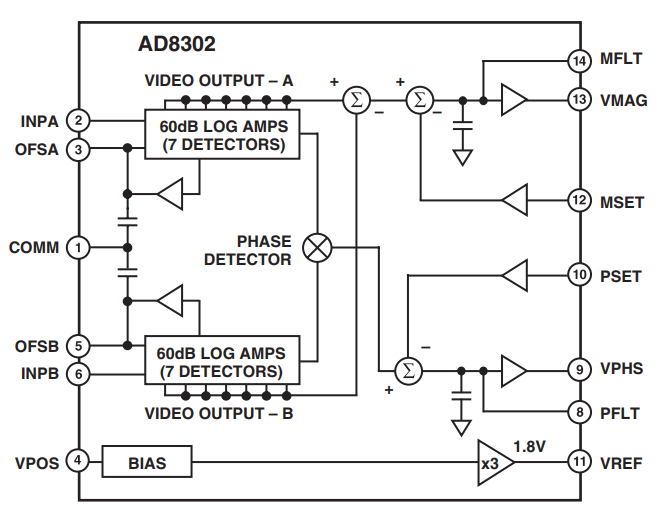
\includegraphics[width=0.8\linewidth]{ad8302_blockdiagram.png}
	\caption{Functional Block Diagram of AD8302}
	\label{fig:ad8302_block_diag}
\end{figure}

Given RF inputs on INPA and INPB, the AD8302 outputs two analog signals ranging from 0 to 1.8V on VMAG and VPHS which correspond to the gain and phase difference between the two RF signals. However these outputs are not perfect, and as such there are various considerations which need to be taken into account to ensure that the gain and phase differences are represented accurately. 

\textbf{VMAG Log Conformance Error} \\
The VMAG output of the AD8302 shown in Figure \ref{fig:ad8302_VMAG_conformance}, which represents the magnitude ratio of the two RF inputs, has decreased linearity towards the ends of its span. Although this could be compensated for through using a non linear model for the voltage to gain conversion, given that the error exceeds 0.5 dB at $\pm$27 dB, which is not only enough dynamic range for many measurements but only 3 dB from the limits of the output, it will not be compensated for due to the limited time available for this project.  
\begin{figure}[H]
	\centering
	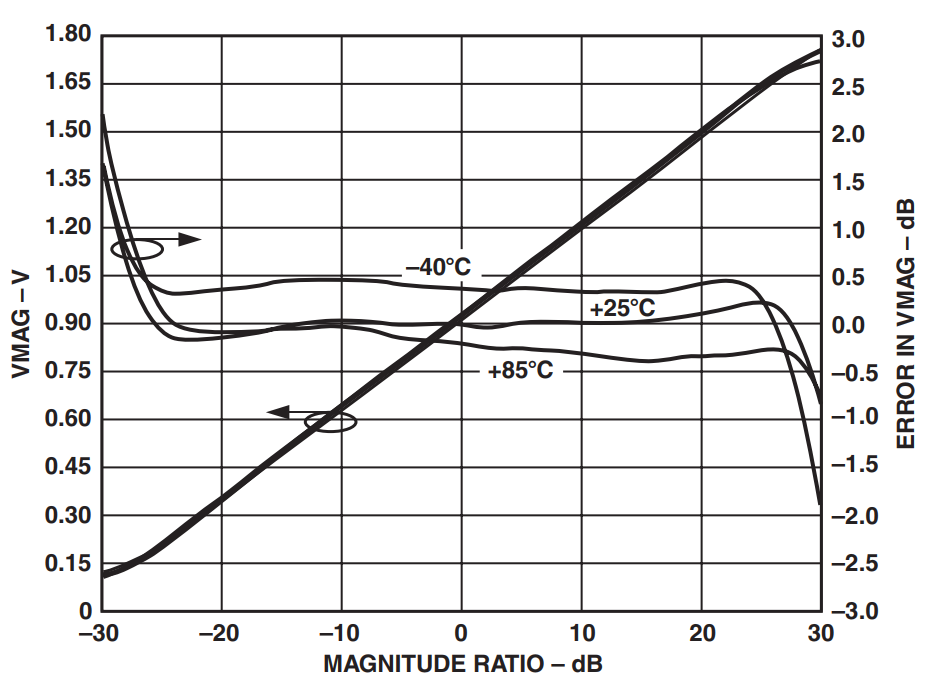
\includegraphics[width=0.6\linewidth]{ad8302_gain_conformance_error.png}
	\caption{VMAG Log Conformance Error}
	\label{fig:ad8302_VMAG_conformance}
\end{figure}

\textbf{VPHS Sign Ambiguity} \\
As shown in Figure \ref{fig:ad8302_VPHS_frequency}, the output voltage representing the phase difference is unable to differentiate between positive and negative phase, due to the output voltage being symmetrical around zero phase difference. It should however be noted that the gradient between -180 and 0 phase is different to 0 to +180 degrees, and as such by looking at how the phase changes as a function of frequency the sign of phase can be determined. The implementation of the signal processing required to make this determination will be explained in \S \ref{sec:implementation}. 
\begin{figure}[H]
	\centering
	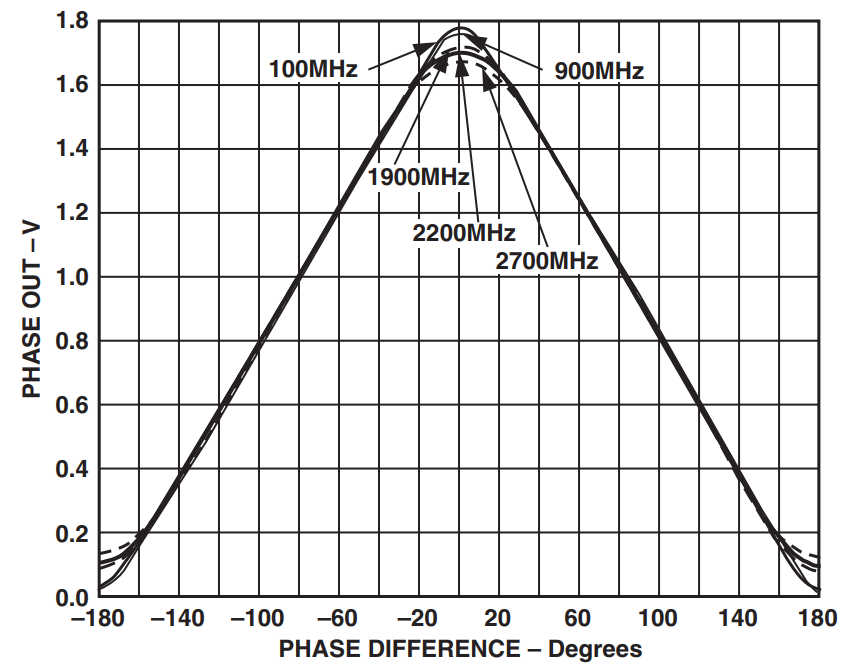
\includegraphics[width=0.6\linewidth]{ad8302_phase_frequency.png}
	\caption{VPHS Output over Frequency and Phase}
	\label{fig:ad8302_VPHS_frequency}
\end{figure}

\textbf{VPHS Log Conformance Error}\\
Like VMAG, VPHS has log conformance errors at the limits of the internal detectors, which manifest in increased errors when the phase difference is small between the two signals. This is highlighted in Figure \ref{fig:ad8302_VPHS_conformance}, which shows the phase error at 900 MHz can be up to 8 degrees when comparing the actual voltage output to the ideal linear fit. Measuring this flattening out of the output voltage and ensuring that the resolution of the sampling ADC is sufficiently high that it can detect the difference at low phase difference values is crucial, as this would allow reconstruction of the actual phase output with sufficient signal processing, which will be outlined in \S \ref{sec:implementation}. 
\begin{figure}[H]
	\centering
	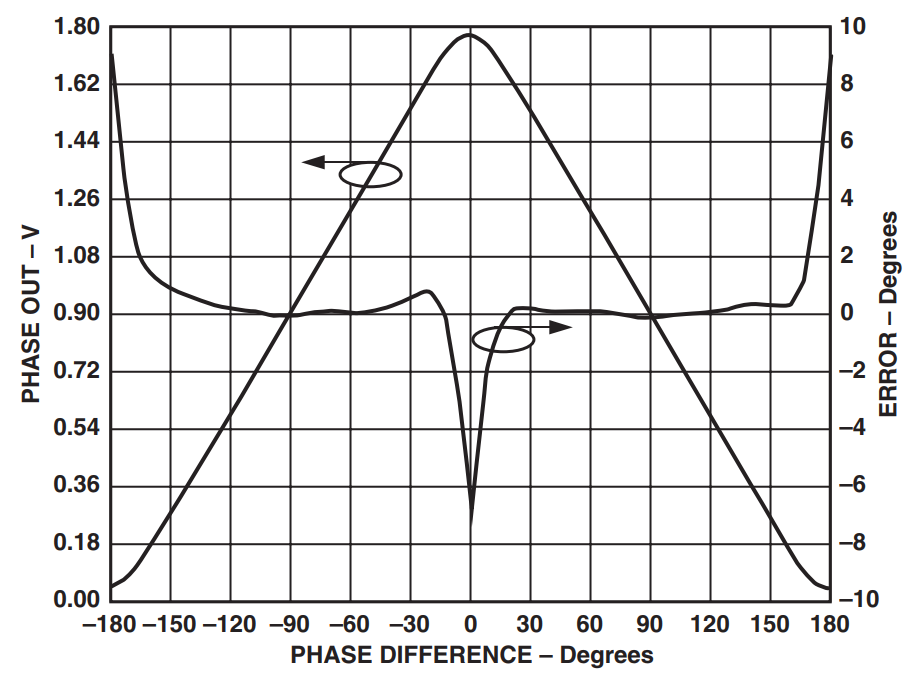
\includegraphics[width=0.6\linewidth]{ad8302_phase_error.png}
	\caption{VPHS Log Conformance Error at 900 MHz}
	\label{fig:ad8302_VPHS_conformance}
\end{figure}

\textbf{VPHS Frequency Dependence} \\
It should also be noted that as shown in Figure \ref{fig:ad8302_VPHS_frequency}, the log conformance error increases as a function of frequency. This will need to be compensated for in addition to the error increasing at small phase differences, and this will be covered in \S \ref{sec:implementation}. 

\subsubsection{Processor}
Sampling of the ADC, control of all onboard devices, along with communications with the host machine will require an embedded processor. As such, a microcontroller with sufficient pins and peripherals to connect to all required hardware, along with inbuilt USB and DSP instructions would be ideally suited to the task. Furthermore, an integrated ADC with at least 12 bits would be ideal, as this would ensure that sampling of the AD8302 could be done with the accuracy required. The STM32F373 series from STMicroelectronics is a great fit for this, as the line-up has 16 bit sigma-delta ADCs with programmable gain, a Cortex-M4 core which has DSP instructions capable of floating point add, multiply, and subtraction in a single clock, along with 64 to 256 Kbytes of flash, and packages with between 48 and 100 pins which will allow the hardware to scale once final specifications and code size are determined. 

\subsubsection{Power}
With components selected, it was determined that 100mA would be required at 5V, with approximately 300mA at 3V3 to power the devices. Due to the supply being 5V from USB, and the desire for low noise power rails due to the sensitive RF and analog measurements occurring, linear regulators were chosen to regulate the power down to 3V3 due to the low input voltage difference and desire for low output ripple. In particular, the LP5912 from Texas Instruments was chosen due to it's low output noise of 12$\mu$V\textsubscript{RMS} and high PSRR of 75dB at 1kHz, whilst costing less than \$2 in singles. Furthermore, the 3V3 rail was divided into analog and digital domains, with separate regulators for each and ferrite beads being used throughout to further reduce the influence of power supply noise on the system. 

\subsection{Firmware and Software}
\label{subsec:firmware_software}
Originally it was planned that the VNA would be a self contained device, capable of all correction and calibration required on device, and would expose itself via a serial port over which it could be controlled and calibrated data returned. However due to the complexity of this architecture and the time constraints on the project, most of the correction and calibration was moved over to the host computer, where Python tools such as NumPy, SciPy, and scikit-rf could be utilised to decrease the development time required, along with allowing decreased compute power for the embedded processor which would help reduce cost. 

Figure \ref{fig:sw_flowchart} shows the primary functions implemented in Software / Firmware, with the blue functions implemented host side in Python, and the purple functions running on the microprocessor in C. The interface between the two sides is done in plain text, and as such the VNA is capable of being controlled over a serial port if desired, with it returning a non calibrated, non phase corrected frequency / magnitude / phase triplet, which could be copied from the terminal and processed as desired. Further detail of the primary functional blocks will be discussed in \S \ref{sec:implementation}, as the architecture was developed during board bring-up and implementation. 

\begin{landscape}
	\begin{figure}[H]
		\centering
		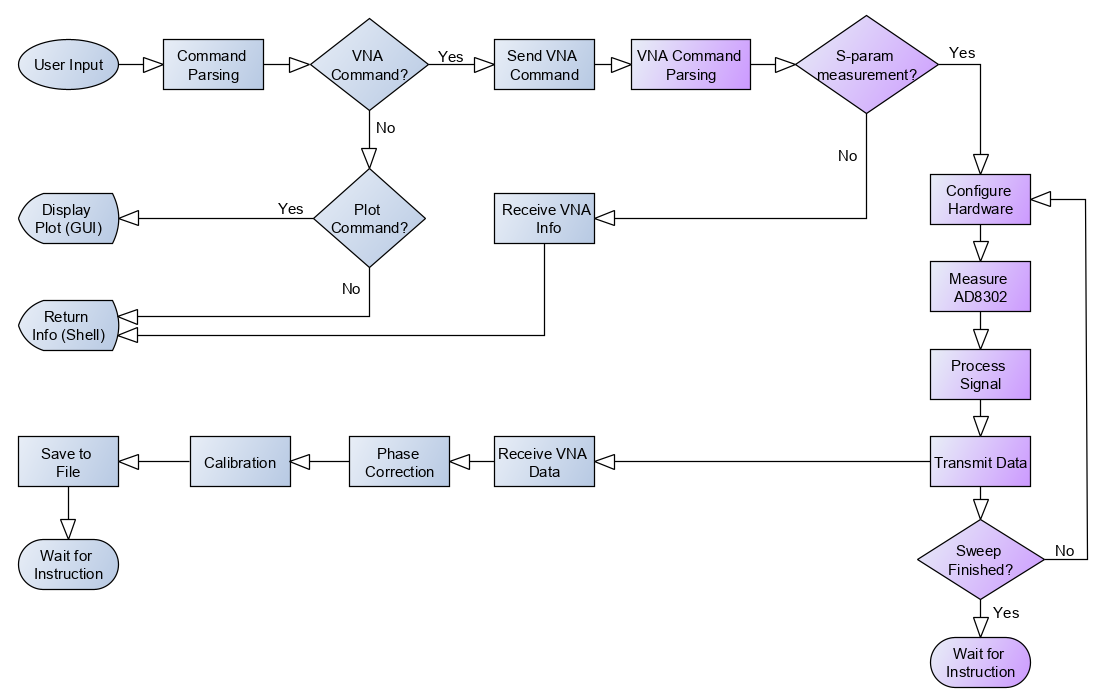
\includegraphics[width=\linewidth]{sw_flowchart.png}
		\caption{Flowchart of Primary Software / Firmware Steps}
		\label{fig:sw_flowchart}
	\end{figure}
\end{landscape}